%%%%%%%% DOCUMENT PREAMBLE %%%%%%%%
\documentclass[man]{apa7}
% load packages
\usepackage{graphicx} % for using figures and images
\usepackage{setspace} % for setting the line space
\doublespacing
\usepackage{geometry} % for setting page formates
    \geometry{
        a4paper,
        left=1in,
        top=1in
    }
\usepackage{lineno} % for numbering the lines
\linenumbers
\usepackage[style=apa,backend=biber]{biblatex} % for references
\addbibresource{references.bib} % your .bib file. Change if needed.
\usepackage[american]{babel} % for language
\usepackage{lipsum} % For template formatting. Remove when writing.
\usepackage{import} % for connecting files to main.tex
%%%%%%%%%%%%%%%%%%%%%%%%%%%%%%%%%%%

%%%%%%% TITLE PAGE PREAMBLE %%%%%%%
\shorttitle{Sample Short title}
\title{Sample Regular Long Title}
% \author{Your Name} % for 1 author
\authorsnames{Author One, Author Two} % for 2 authors
\affiliation{Department of $\LaTeX$} % for 1 affiliation
% \authorsaffiliations{{Department of $\LaTeX$}, {Department of Psychology}} % for multiple affiliations
\authornote{
    \addORCIDlink{Your Name}{0009-0000-0000-0000}
    
All correspondence concerning this article should be addressed to Your Name,
Department of $\LaTeX$
}
\abstract{
\lipsum[1]
}
\keywords{KW1, KW2, ...}
%%%%%%%%%%%%%%%%%%%%%%%%%%%%%%%%%%%

%%%%%%% BEGIN MAIN DOCUMENT %%%%%%%
\begin{document}
    \maketitle

\lipsum[1-2] % for filling space. Delete.
\subsection{Subsection One}
%%%%%%%%% Sample Figure %%%%%%%%%%
\begin{figure}[h!]
    \centering
    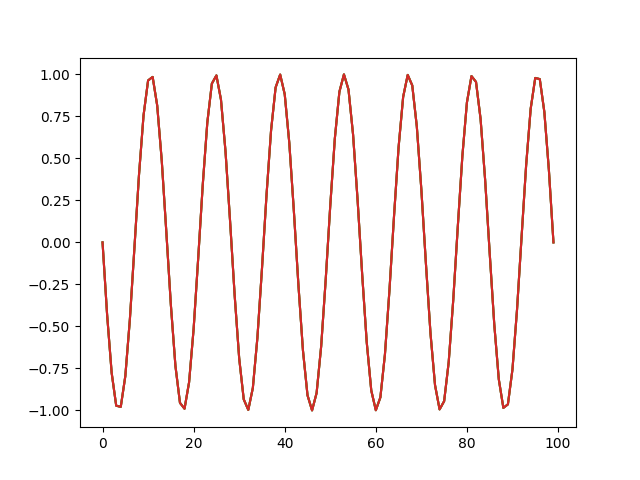
\includegraphics[scale=0.4]{figures/sinewave.png}
    \caption{Sine Wave}
    \label{fig:sinwave}
\end{figure}
%%%%%%%%%%%%%%%%%%%%%%%%%%%%%%%%%%%
\lipsum[1] % for filling space. Delete.
\section{Methods}
\lipsum[2]

\printbibliography

\end{document}



